\section{Caracterización de celdas}
Se construyen tres celdas de distintas dimensiones para analizar la dependencia de las dimensiones de la celda con su respuesta en frecuencia. Estas se observan en la figura \ref{fig:celdas}.\\

Las celdas se encuentran numeradas y sus lados nombrados, distancia entre electrodos (l), ancho (a) y altura (h). En el cuadro \ref{tabla:celdas_dimen} se observan las dimensiones de las mismas.\\

\begin{figure}[H]
\centering
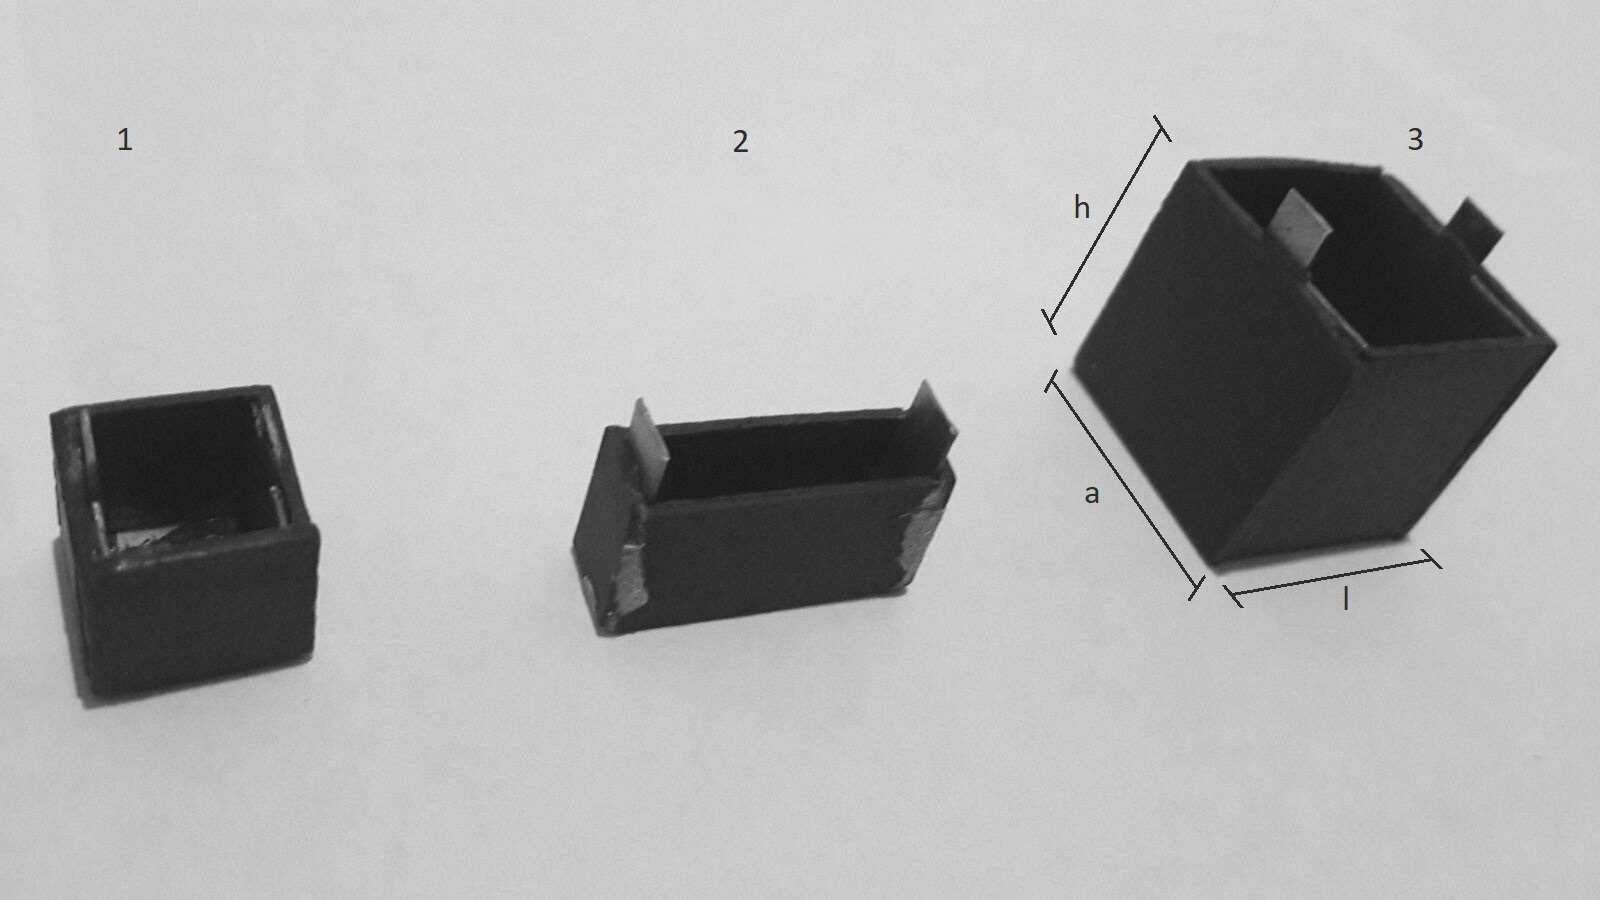
\includegraphics[width=1\textwidth]{Celda/celdas_num.jpg}
\caption{Celdas de ensayo}
\label{fig:celdas}
\end{figure}

\begin{table}[htp]
\centering
\caption{Dimensiones de las celdas}
\label{tabla:celdas_dimen}

\begin{tabular}{|l|l|l|l|}
	\hline
	Celda & l (cm) & a (cm)& h (cm)  \\ \hline
	1 & 0,9 & 1,0 & 1,0\\ \hline
    2 & 2,0 & 0,5 & 1,0\\ \hline
    3 & 1,9  & 2,0 & 2,1\\ \hline
 
\end{tabular}
\end{table}

Se construyen las celdas con plástico y los electrodos con placas de acero inoxidable para que los químicos de limpieza no las corroan.\\

En REFERENCIA, se modela la celda con el modelo equivalente eléctrico observado en la figura \ref{fig:celda_eq}, donde $C_{pp}$ es la capacidad placa-placa, $C_{pm}$ es la capacidad equivalente de las dos capacidades placa-leche y $R_{m}$ es la resistencia de la leche que es la que se desea medir.\\

\begin{figure}[H]
\centering
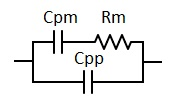
\includegraphics[width=0.3\textwidth]{Celda/celda_eq.jpg}
\caption{Circuito equivalente de celda con leche}
\label{fig:celda_eq}
\end{figure}

En las figuras \ref{fig:celda_1}, \ref{fig:celda_2} y \ref{fig:celda_3} se gráfica la resistencia $R_{m}$ y la fase de la impedancia en función de la frecuencia para cada una de las celdas.\\

Al observar las fases de las tres celdas se aprecia un comportamiento principalmente capacitivo a baja frecuencia, un comportamiento resistivo a frecuencia intermedia y nuevamente comportamiento capacitivo a alta frecuencia. Esto se debe a que para estas dimensiones de celdas la capacidad $C_{pp}$ es más chica que la $C_{pm}$(COMENTAR PORQUE. DISTANCIA). Como la impedancia de un capacitor crece al bajar la frecuencia, a frecuencia baja domina la impedancia de $C_{pm}$ sobre $R_{m}$. A medida que la frecuencia sube empieza a dominar $R_{m}$ hasta el punto en que la impedancia de $C_{pp}$ en paralelo se achica lo suficiente que domina sobre ambas.\\

Dado que el circuito de medición mide el módulo de la impedancia, se  desea que éste sea lo más parecida a $R_{m}$. Observando las figuras, se aprecia que el punto óptimo es a 100 kHz, ya que en este punto el comportamiento es principalmente resistivo. Además en un entorno de esta frecuencia $R_{m}$ se mantiene constante, pero cuanto más alta es la frecuencia más requerimientos trae sobre el circuito. Por otro lado, en el caso de la celda 2, el desfasaje a 100 kHz es -5.17 grados y a 10 kHz es de -5.58 grados. Por esto, se decide utilizar la celda 2 a una frecuencia de trabajo de 10 kHz.\\

\begin{figure}[H]
\centering
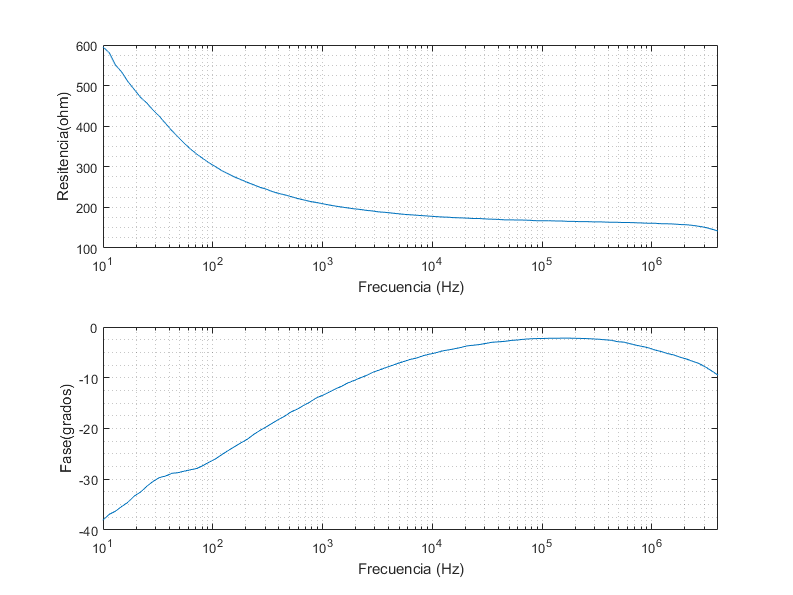
\includegraphics[width=1\textwidth]{Celda/celda_1.png}
\caption{Resistencia y fase en función de la frecuencia para la celda 1}
\label{fig:celda_1}
\end{figure}

\begin{figure}[H]
\centering
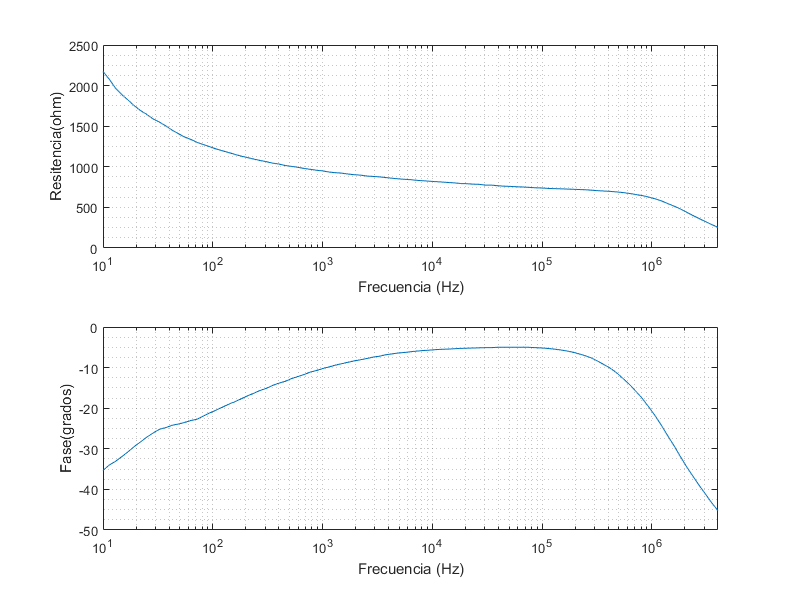
\includegraphics[width=1\textwidth]{Celda/celda_2.png}
\caption{Resistencia y fase en función de la frecuencia para la celda 2}
\label{fig:celda_2}
\end{figure}

\begin{figure}[H]
\centering
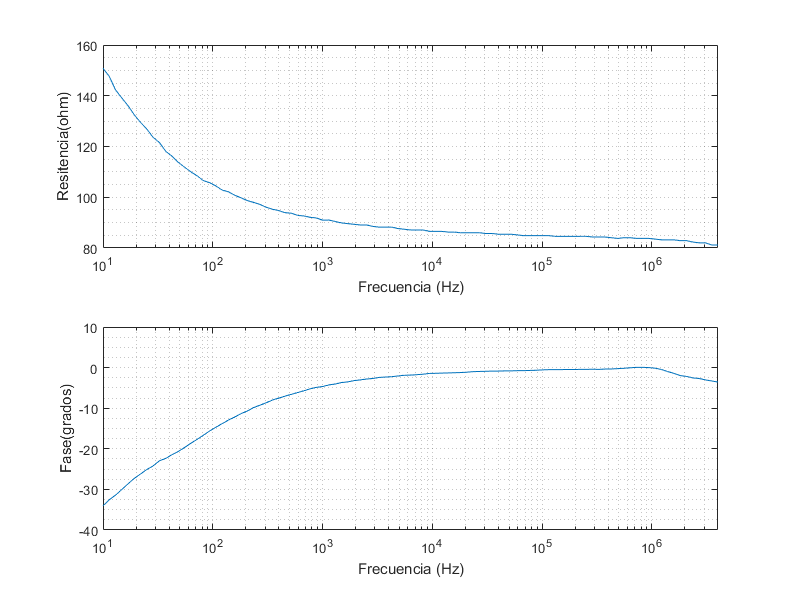
\includegraphics[width=1\textwidth]{Celda/celda_3.png}
\caption{Resistencia y fase en función de la frecuencia para la celda 3}
\label{fig:celda_3}
\end{figure}

En el cuadro \ref{tabla:celdas_error} se presenta la resistencia, la impedancia y el cálculo del error relativo de tomar como medida de $R_{m}$ el módulo de la impedancia $error=\dfrac{|Z|-R_{m}}{R_{m}}\times 100$ \\
Los valores fueron relevados a 10kHz y $27^{o}C$
\begin{table}[htp]
\centering
\caption{Comparación entre el módulo de la impedancia y la resistencia}
\label{tabla:celda_error}

\begin{tabular}{|l|l|l|l|}
	\hline
	Celda &$|Z|(\Omega)$& $R_{m}(\Omega)$& error(\%)  \\ \hline
	1 & 178,1& 177,4 & 0.39\\ \hline
    2 & 821,4 & 817,5 & 0.48\\ \hline
    3 & 86,58  & 86,56 & 0.02\\ \hline
 
\end{tabular}
\label{tabla:celdas_error}
\end{table}

Si se comparan los errores la peor celda es la 2 pero de todos modos el error es muy bajo ($0.48\%$) y ésta tiene una ventaja sobre las demás que es que la resistencia $R_{m}$ es casi un orden más grande, lo que como se vera más a delante le otorga mas sensibilidad a la medida.\\

Con $R_{m}$ y las dimensiones de cada celda se puede calcular tres estimadores de la conductividad media de la leche a $27^{o}C$ ya que la leche se extrajo del tanque de  frío que tiene la leche de todas las vacas mezcladas.\\

Se sabe que $R_{m}=\dfrac{l}{\sigma .S}$ donde S es la sección de la placa entonces:\\

\begin{equation}
\sigma=\dfrac{l}{R_{m}.a.h}
\end{equation}

En el cuadro \ref{tabla:sigma} se muestran los tres valores de $\sigma$. Promediando se obtiene: $\sigma=5.06 mS/cm$
\begin{table}[htb]

\centering
\caption{Cálculo de conductividad}
\label{tabla:sigma}
\begin{tabular}{|l|l|l|l|}
\hline
$\sigma (mS/cm)$ &5,07 & 4,89 &5,23\\ \hline

\end{tabular}

\end{table}

La conductividad crece linealmente con la temperatura según la ecuación \ref{eq:sigma}.\\

\begin{equation}
\sigma=\sigma_{o}(1+\alpha(T-T_{o}))
\label{eq:sigma}
\end{equation}

Se desea calcular el parámetro $\alpha$ para realizar las correcciones pertinentes al tomar cada medida.\\

Despejando $\alpha$ de la ecuación \ref{eq:sigma} y sustituyendo $\sigma =\frac{1}{R_{m}}$ se llega a la ecuación \ref{eq:alfa}\\

\begin{equation}
\alpha=\dfrac{1}{T-T_{o}}\left(\dfrac{R_{mo}}{R_{m}}-1\right)
\label{eq:alfa}
\end{equation}

Para calcular $\alpha$ se relevó la resistencia $R_{m}$ de la celda 2 a 10kHz y a tres temperaturas distintas como se muestra en la tabla \ref{tabla:alfa}.

\begin{table}[htb]

\centering
\caption{Rm a distintas temperaturas}
\label{tabla:alfa}
\begin{tabular}{|l|l|l|l|}
\hline
T (°C)& $R_{m}(\Omega)$ \\ \hline
 27& 817 \\ \hline
 31& 743 \\ \hline
 35& 674 \\ \hline
\end{tabular}

\end{table}

Con estos datos se puede calcular tres estimadores de alfa.

\begin{table}[htb]

\centering
\caption{Cálculo de alfa}

\label{tabla:alfa2}
\begin{tabular}{|l|l|l|l|}
\hline
$\alpha (\%)$ &2,49 & 2,56 &2,65\\ \hline

\end{tabular}

\end{table}

Promediando se obtiene $\alpha(\%)=2.57$